% !TEX root = ../main.tex
\newpage
% Раздел 3
\section{Реализация}\label{sec:razd3}

% \subsection{Технология реализации} % ?
% ООП
% выбор языков программирования
% используемые библиотеки/модули
% git
%% работа с репозиторием
%% commitы

\subsection{Общее описание проекта} % ?
% Общее описание разработанного проекта
% Общее описание структуры проекта

Согласно поставленным задачам, проект должен содержать:
\begin{itemize}
  \item Реализацию алгоритмов шифрования;
  \item Модуль для работы с зашифрованными файлами;
  \item Описание пользовательского интерфейса;
  \item Файлы локализаций.
\end{itemize}

Для удобного взаимодействия разработчика с проектом,
была использована система контроля версий Git.
Структура репозитория была определена следующим образом:

\verbatiminput{./cont/app-raw-tree-desc.txt}

\emph{Алгоритмы шифрования} подключаются к программе как динамические
библиотеки. Реализация каждого алгоритма шифрования содержится в своей
директории отдельно от остальных исходников.

\emph{Модули программы} поделены на несколько частей:
\begin{itemize}
    \item Привязка динамических библиотек с алгоритмами шифрования к Python;
    \item Модуль для работы с разработанным форматом файла;
    \item Описание логики работы графического пользовательского интерфейса.
\end{itemize}

\emph{Файлы локализаций} содержат перевод строк, используемых в приложении:
`Файл', `правка', `сохранить', `копировать', `вставить' и т. д.

% сюда бы водички

Весь исходный код проекта содержится в репозитории на GitHub.
Веб-адрес репозитория: \verb'http://github.com/MrP4p3r/PyTFE'.

\newpage
Далее представлено содержание проекта на финальной стадии разработки:

\verbatiminput{./cont/app-tree.txt}

\newpage
\subsection{Реализация алгоритмов шифрования} % ?

Существуют различные режимы шифрования исходного текста блочным
шифром: режим простой замены (ECB), режим сцепления блоков (CBC),
режим обратной связи по шифротексту (CFB), режим обратной связи по
выходу (OFB) и др. Несмотря на явные недостатки режима ECB,
из-за простоты реализации был выбран именно он.

При выполнении работы были написаны реализации алгоритмов шифрования
FEAL-4 и Blowfish на языке ассемблера и на языке высокого уровня C.
Исходный код всех реализаций представлен в приложении А.

Для компиляции исходного кода на языке C был использован компилятор
GNU C Compiler (\texttt{gcc}),
для компиляции ассемблерного кода -- Flat Assembler (\texttt{fasm}).
Был проведен анализ скорости шифрования каждой из реализаций. Результаты
приведены в таблице \ref{tab:enc-speed-rez}.

\noindent
\begin{minipage}{\linewidth}
  \vspace{2.5mm}
  \captionof{table}{Результаты сравнения скорости работы алгоритмов}\label{tab:enc-speed-rez}
  \vspace{-2.5mm}
  \begin{tabular}{|l|l|l|l|}
    \hline
    Шифр            & Скорость шифрования/дешифрования \\\hline
    Blowfish (C)    & 151.7 Мб/с  \\\hline
    Blowfish (ASM)  & 108.4 Мб/с  \\\hline
    FEAL-4 (C)      & 234.3 Мб/с  \\\hline
    FEAL-4 (ASM)    & 382.4 Мб/с  \\\hline
  \end{tabular}
  \vspace{2.5mm}
\end{minipage}\\

Скорость выполнения кода на языке C зависит от качества оптимизаций,
которые проводит компилятор. А скорость выполнения ассемблерного кода
прямо зависит от исходного кода, поскольку выполняется лишь трансляция
в машинный код.

Результаты сравнения скорости работы реализаций алгоритмов получились
несколько противоречивыми: FEAL-4, написанный на языке C, работает медленнее
неоптимизированной ассемблерной реализации, в то время как Blowfish работает
быстрее реализации на языке ассемблера, код которой был написан
относительно аккуратно.

В любом случае, переносимость кода все-таки перевешивает несущественное
уменьшение производительности одного из алгоритмов. Поэтому в качестве
основных реализаций алгоритмов, которые будут использованы в программе,
были выбраны реализации на языке C.

Исходный код был скомпилирован компилятором GNU C Compiler в динамические
библиотеки feal4.dll и blowfish.dll для использования в программе.

\newpage
\subsection{Связка динамических библиотек с Python}\label{ssec:python-algo-bindings} % ?

Подключение модулей в Python осуществляется оператором \texttt{import}.
Однако таким образом могут быть подключены лишь модули, написанные
на Python. Для подключения динамических библиотек в Python
используется модуль ctypes.

В ctypes имеются функции для работы с динамическими библиотеками (.DLL)
в Windows и shared objects (.SO) на UNIX-подобных системах.
Однако в рамках работы была добавлена лишь поддержка DLL.

Разработанные динамические библиотеки необходимо связать с функциями
на Python. Для удобства обращения к этим функциям, они были оформлены
как методы классов. Каждый класс имеет одинаковый интерфейс (набор методов):
функции шифрования/дешифрования чанка, шифрования/дешифрования
одного блока и конструктора класса. Это позволяет упростить реализацию
общей функции шифрования: ее реализация не зависит от определенного
алгоритма шифрования.

Связка динамических библиотек с Python состоит из двух модулей:
\texttt{feal4.py} и \texttt{blowfish.py} (код модулей можно найти в приложении Б).
В них содержатся описания классов feal4 и blowfish. При инициализации
экземпляров класса необходимо задать секретный ключ, по которому будет
производиться шифрование. После этого можно начинать использовать использовать
объекты через вышеописанный интерфейс.

\newpage
\subsection{Модуль для работы с зашифрованными файлами} % ?

Для шифрования и упаковки данных пользователя был разработан отдельный
модуль, на языке Python (исходный код имеется в приложении Б).
Модуль содержит набор констант, таблицы алгоритмов шифрования и хэширования
и набор базовых функций для работы с форматом, таких как формирование/чтение
заголовка файла, шифрование/дешифрование буфера
\footnote{Буфер -- (здесь) объект имеющий интерфейс, позволяющий производить
операции чтения, записи, установки курсора и т. д. Буфером может быть открытый
файл или строка в памяти.},
шифрование/дешифрование файлов.

Таблица алгоритмов шифрования для каждого алгоритма имеет
указатель на класс (пункт \ref{ssec:python-algo-bindings}),
функцию генерации ключа, размер блока функции шифрования,
размер чанка (считываемого блока данных из буфера) и идентификатора алгоритма.
Формат предусматривает наличие до 256-ти записей в таблице алгоритмов.
Таблица алгоритмов хэширования содержит функцию хэширования, длину хэша
и идентификатор соответствующие алгоритму хэширования. Алгоритмов хэширования
в таблице также может быть до 256-ти.

Использование модуля в целом сводится к вызову функций шифрования и
дешифрования буферов при сохранении и чтении файла соответственно.
Функция шифрования принимает на вход указатель на входной буфер,
выходной буфер, длину входного буфера, символьный пароль и опционально
алгоритм шифрования и алгоритм хэширования в соответствии с вышеописанными
таблицами. По умолчанию используются алгоритмы Blowfish и MD5 для
шифрования и хэширования соответственно.
Функция дешифрования принимает на вход указатель на входной буфер с
зашифрованными данными, выходной буфер для расшифрованных данных и
символьный пароль.

Для генерации ключей по символьному паролю используется алгоритм PBKDF2.
Алгоритм позволяет генерировать ключ произвольной длины по символьому
паролю произвольной длины. То есть этот алгоритм можно использовать в
связке с любым алгоритмом шифрования. Алгоритм позволяет ``разбавлять''
символьный пароль т. н. солью. Соль хранится вместе с зашифрованными данными.
В работе была использована сторонняя реализация алгоритма, поэтому
подробно его работа не рассмотрена.

\newpage
\subsection{Реализация графического интерфейса} % ?

Пакет Qt5 предлагает утилиту QtDesigner для проектирования
графического интерфейса. Но в качестве альтернативы интерфейс может быть
описан в коде программы без использования QtDesigner. Именно так и было
сделано, поскольку в этом есть ряд преимуществ для автора работы.

Описание графического интерфейса представляет собой несколько Python-скриптов
с переназначением некоторых базовых классов библиотеки Qt5 и набора методов:
\begin{enumerate}
    \item \texttt{interte.py}\\
    Скрипт содержит переопредление класса виджета QMainWindow --
    главного окна программы (рисунок \ref{fig:app-main-window}),
    и набор методов, реализующих основные функции типичного текстового редактора.
    \item \texttt{mwidgetste.py}\\
    Скрипт содержит дополнительные переопределенные виджеты, а также
    описание окна настроек программы
    (рисунки \ref{fig:app-settings-window-1}-\ref{fig:app-settings-window-2}).
    \item \texttt{defaultvalues.py}\\
    Скрипт содержит определения констант.
\end{enumerate}

\noindent
\begin{minipage}{\linewidth}
  \vspace{3.5mm}
  \centering
  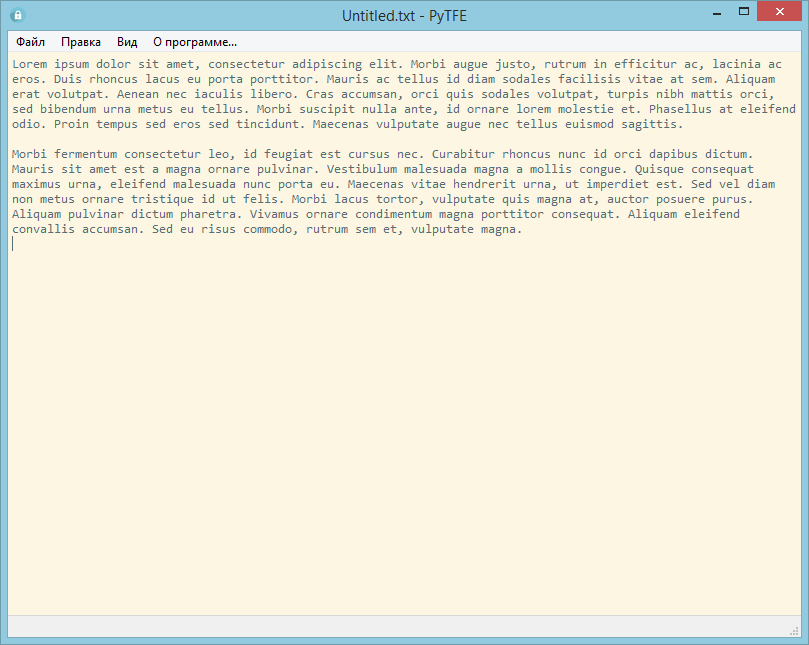
\includegraphics[scale=0.6]{./pics/te/app-main-window.png}
  \captionof{figure}{Вид главного окна программы}\label{fig:app-main-window}
  \vspace{3.5mm}
\end{minipage}

\noindent
\begin{minipage}{\linewidth}
  \vspace{3.5mm}
  \centering
  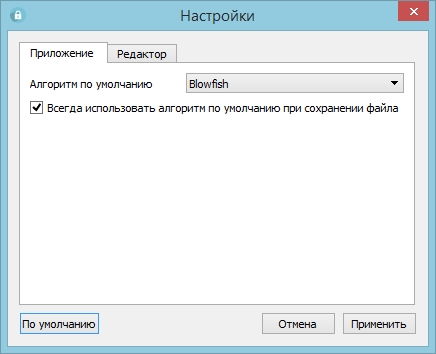
\includegraphics[scale=0.6]{./pics/te/app-settings-window-1.png}
  \captionof{figure}{Вид окна настроек: основные настройки}\label{fig:app-settings-window-1}
  \vspace{3.5mm}
\end{minipage}

\noindent
\begin{minipage}{\linewidth}
  \vspace{3.5mm}
  \centering
  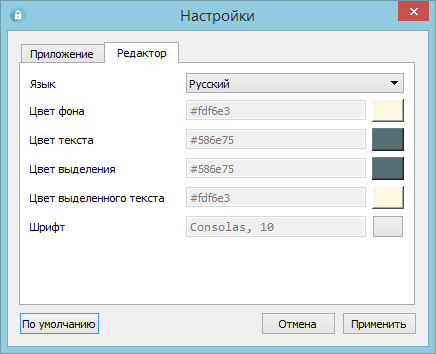
\includegraphics[scale=0.6]{./pics/te/app-settings-window-2.png}
  \captionof{figure}{Вид окна настроек: настройки редактора}\label{fig:app-settings-window-2}
  \vspace{3.5mm}
\end{minipage}

\subsection{Перевод приложения}

Библиотека Qt5 имеет средство для интернационализации (перевода) приложений.
С помощью утилиты \texttt{lupdate} создаются файлы локализаций,
которые содержат перевод строк в графическом интерфейсе в формате XML.
Редактирование файлов локализаций (перевод приложения)
осуществляется утилитой \texttt{linguist}. Утилита \texttt{lrelease} позволяет
``скомпилировать'' файлы локализаций для использования в готовом приложении.

В разработанной программе имеется поддержка
русского (рисунок \ref{fig:app-russian})
и английского (рисунок \ref{fig:app-english}) языка.

\noindent
\begin{minipage}{\linewidth}
  \vspace{3.5mm}
  \centering
  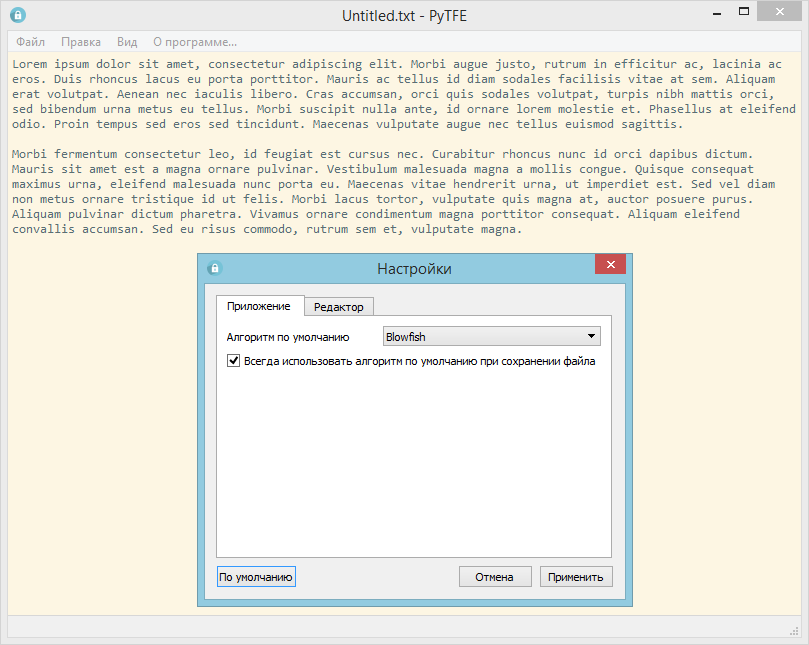
\includegraphics[scale=0.6]{./pics/te/app-russian.png}
  \captionof{figure}{Русский графический интерфейс}\label{fig:app-russian}
  \vspace{3.5mm}
\end{minipage}

\noindent
\begin{minipage}{\linewidth}
  \vspace{3.5mm}
  \centering
  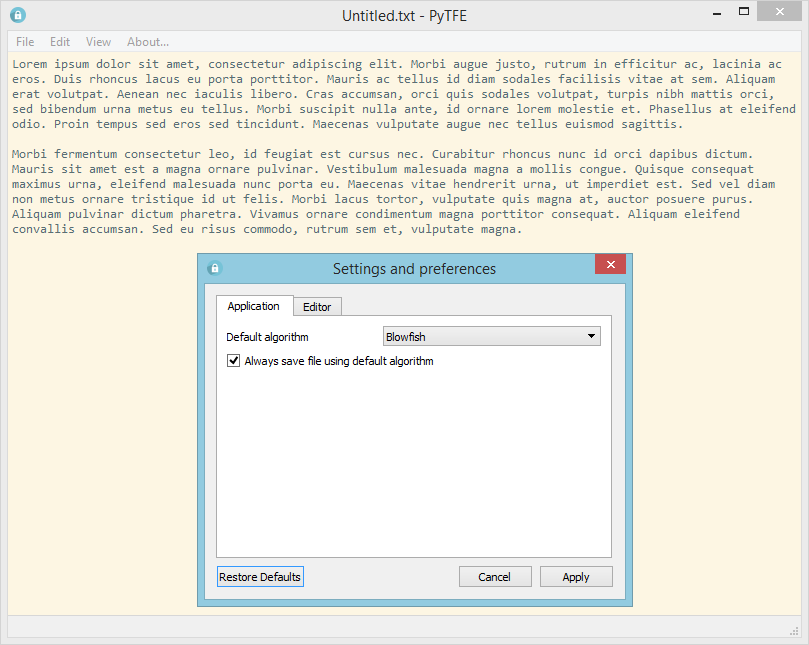
\includegraphics[scale=0.6]{./pics/te/app-english.png}
  \captionof{figure}{Английский графический интерфейс}\label{fig:app-english}
  \vspace{3.5mm}
\end{minipage}
